\documentclass[10pt]{article}

\usepackage{amsthm}
\usepackage[toc,page]{appendix}
\usepackage{amssymb}
\usepackage{bm}
\usepackage{pslatex,palatino,avant,graphicx,color}
\usepackage{colortbl}
\usepackage{fullpage}
\usepackage{mathtools}
\usepackage{natbib}
\usepackage{amsmath}
\usepackage{caption}
%\usepackage{subfigure}
\usepackage{subcaption}
\usepackage{bm}
\usepackage{wrapfig}
\usepackage{enumerate}
\usepackage{rotating}
\usepackage{multirow}
\usepackage{tabularx}
\usepackage{tikz}
\usepackage{pgfplots}
\usepackage{bbm}
\usepackage[titles,subfigure]{tocloft} % Alter the style of the Table of Contents

\newtheorem{lemma}{Lemma}
%\pdfminorversion=4
% NOTE: To produce blinded version, replace "0" with "1" below.
\newcommand{\blind}{0}

% DON'T change margins - should be 1 inch all around.
\addtolength{\oddsidemargin}{0in}%
\addtolength{\evensidemargin}{0in}%
\addtolength{\textwidth}{0in}%
\addtolength{\textheight}{0in}%
\addtolength{\topmargin}{0in}%


\renewcommand{\cftsecfont}{\rmfamily\mdseries\upshape}
\renewcommand{\cftsecpagefont}{\rmfamily\mdseries\upshape} % No bold!

\newcommand{\indicator}[1]{\mathbbm{1}\left( #1 \right) }
\newcommand{\hb}{\hat{b}}
\newcommand{\ha}{\hat{a}}
\newcommand{\htheta}{\hat{\theta}}
\newcommand{\halpha}{\hat{\alpha}}
\newcommand{\hmu}{\hat{\mu}}
\newcommand{\hsigma}{\hat{\sigma}}
\newcommand{\hphi}{\hat{\phi}}
\newcommand{\htau}{\hat{\tau}}
\newcommand{\heta}{\hat{\eta}}
\newcommand{\E}[1]{\mbox{E}\left[#1\right]}
\newcommand{\Var}[1]{\mbox{Var}\left[#1\right]}
\newcommand{\Indicator}[1]{\mathbbm{1}_{ \left( #1 \right) } }
\newcommand{\dNormal}[3]{ N\left( #1 \left| #2, #3 \right. \right) }
\newcommand{\Beta}[2]{\mbox{Beta}\left( #1, #2 \right)}
\newcommand{\alphaphi}{\alpha_{\hphi}}
\newcommand{\betaphi}{\beta_{\hphi}}
\newcommand{\expo}[1]{ \exp\left\{ #1 \right\}}
\newcommand{\tauSquareDelta}{\htau^2
  \left(\frac{1-\expo{-2\htheta\Delta}}{2\htheta} \right)}
\newcommand{\mumu}{\mu_{\hmu}}
\newcommand{\sigmamu}{\sigma^2_{\hmu}}
\newcommand{\sigmamuexpr}{\log\left( \frac{\VarX}{\EX^2} + 1 \right)}
\newcommand{\mumuexpr}{\log(\EX) -  \log\left( \frac{\VarX}{\EX^2} + 1 \right) /2 }

\newcommand{\EX}{\mbox{E}\left[ X \right] }
\newcommand{\VarX}{\mbox{Var}\left[ X \right] }
\newcommand{\mueta}{\mu_{\heta} }
\newcommand{\sigmaeta}{\sigma^2_{\heta}}
\newcommand{\sigmaetaexpr}{ \log\left( \frac{\VarX}{\EX^2} + 1 \right) }
\newcommand{\muetaexpr}{ \log(\EX) -  \sigmaetaexpr /2 }

\newcommand{\mualpha}{\mu_{\halpha} }
\newcommand{\sigmaalpha}{\sigma^2_{\halpha}}
\newcommand{\sigmaalphaexpr}{ \log\left( \frac{\VarX}{\EX^2} + 1 \right) }
\newcommand{\mualphaexpr}{ \log(\EX) -  \sigmaalphaexpr /2 }

\newcommand{\mutauexpr}{ \frac{2}{T} \EX }
\newcommand{\sigmatauexpr}{ \frac{4}{T^2} \Var{X}}

\newcommand{\alphatau}{\alpha_{\htau^2}}
\newcommand{\betatau}{\beta_{\htau^2}}

\newcommand{\Gam}[2]{\mbox{Gamma}\left( #1, #2 \right) }
\newcommand{\InvGam}[2]{\mbox{Inv-Gamma}\left( #1, #2 \right) }

%%% END Article customizations

%%% The "real" document content comes below...

% \newbox{\LegendeA}
% \savebox{\LegendeA}{
%    (\begin{pspicture}(0,0)(0.6,0)
%    \psline[linewidth=0.04,linecolor=red](0,0.1)(0.6,0.1)
%    \end{pspicture})}
% \newbox{\LegendeB}
%    \savebox{\LegendeB}{
%    (\begin{pspicture}(0,0)(0.6,0)
%    \psline[linestyle=dashed,dash=1pt 2pt,linewidth=0.04,linecolor=blue](0,0.1)(0.6,0.1)
%    \end{pspicture})}

\title{A Range-Based Bivariate Stochastic Volatility Model: Towards Closed-Form Solution}
\author{Georgi Dinolov, Abel Rodriguez, Hongyun Wang}
\date{} % Activate to display a given date or no date (if empty),
         % otherwise the current date is printed

\begin{document}
\def\spacingset#1{\renewcommand{\baselinestretch}%
{#1}\small\normalsize} \spacingset{1}

\bigskip

\vspace{1cm}

In this chapter we develop an analytic solution to the normalized
problem for small $\tilde{\sigma}$ values. We illustrate our approach
with the simple case where $\rho=0$.

\section{A small-parameter analytic solution}
In the previous chapter we introduced a numerical solution that works
for relatively benign parameter ranges. However, the numerical
solution fails for small parameters of $(\tilde{\sigma},
\tilde{t})$. Here, we introduce an analytic solution that works for
certain small-$\tilde{\sigma}$.

\subsection{Illustration with $\rho=0$ and sufficiently small
  $t^{*}$}
Consider the normalized diffusion problem with $\rho=0$
\[
  \frac{\partial q}{\partial t} = \frac{1}{2}\frac{\partial^2 q}{\partial x^2} + \frac{1}{2}\tilde{\sigma}^2 \frac{\partial^2 q}{\partial y^2}.
\]
and an intial condition $(x_0, y_0)$ with absorbing boundaries on the
unit square. The fundamental solution to the problem is an
uncorrelated bivariate Gaussian with variances $t$ and
$t\tilde{\sigma}^2$ in the $x$ and $y$ directions, respectively. The
problem setup and a contour plot of the fundamental solution is
illustrated in Figure (\ref{fig:normalized-problem-rho-0}). As in
Chapter 2, we can scale, rotate, and scale again the problem, so that
the boundaries of the computational domain have changed, but the
fundamental solution to the problem is defined by an uncorrelated
bivariate Gaussian distribution with variance $t$ in each
direction. The transformed problem is shown in Figure
(\ref{fig:transformed-problem-rho-0}).

The topology under the transformed problem permits the fundamental
solution to be translated and rotated without violating the governing
PDE. Hence, we may reflect about the boundaries to enforce the
absorbing condition there while producing a system of images whose sum
satisfies the PDE. In the $\rho=0$ case, the orthogonal angles between
adjecent boundaries ensure that none of the images that result from
repeated reflections fall within the computational domain. This
further allows for subsequent images for fall further from the domain
(scaling linearly in distance) so that we can solve the problem
formally with an infinite number of reflections or semi-analytically
with a finite system of images.
\begin{figure}
  \centering
  %%
  %%
  \begin{tabular}{cc}
    \begin{minipage}{0.40\textwidth}
      \centering
      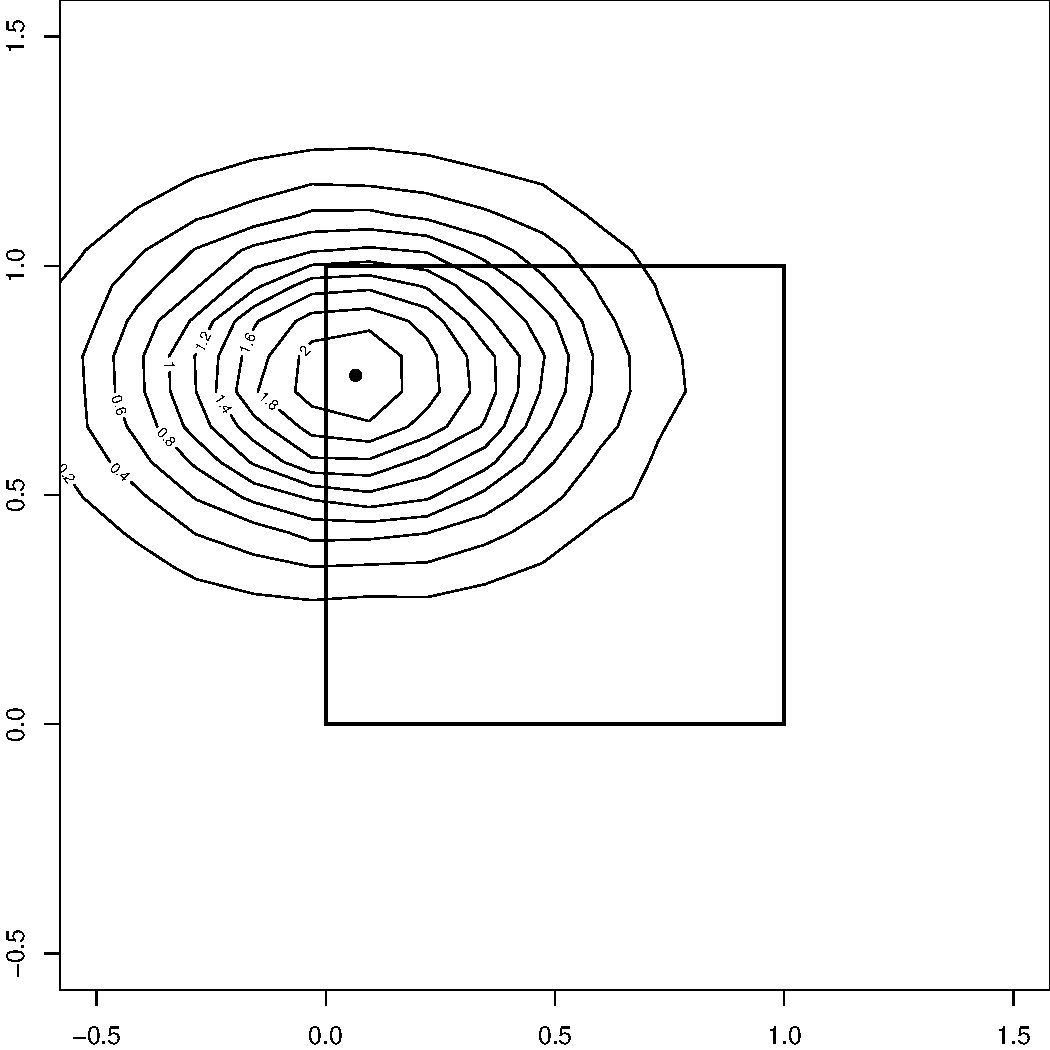
\includegraphics[width=1\linewidth]{illustration-rho-0-normalized.pdf}
      \caption{hello world}
      \label{fig:normalized-problem-rho-0}
    \end{minipage}
    %%
    & \begin{minipage}{0.40\textwidth}
      \centering
      \includegraphics[width=1\linewidth]{illustration-rho-0-transformed.pdf}
      \caption{Small time $\tilde{t} \approx 0.10$.}
      \label{fig:transformed-problem-rho-0}
    \end{minipage}
  \end{tabular}
\end{figure}

We can compose a finite system of images by reflecting about each of
the boundaries a number of times and picking the greatest possible
time $t^{*}$ such that all boundaries are either numerically or
analytically enforced. One candidate for such a set of reflections is
shown in Figure (\ref{fig:illustration-1}), where the set of images is
produced by the reflections (left, right, left, top, bottom, top). The
green points and blue points are image positions differentiable with
respect to all four boundary parameters, where the green points alone
present a symmetric solution about the initial condition (red).

\begin{figure}
  \begin{tabular}{cc}
    \begin{minipage}{0.40\textwidth}
      \centering
      \includegraphics[width=1\linewidth]{chapter-3-figure-illustration-1.pdf}
      \caption{}
      \label{fig:illustration-1}
    \end{minipage}
    %%
    & \begin{minipage}{0.40\textwidth}
      \centering
      \includegraphics[width=1\linewidth]{chapter-3-figure-illustration-rel-error.pdf}
      \caption{}
      \label{fig:illustration-rel-error}
    \end{minipage}
      \end{tabular}
\end{figure}
The resultant approximate \textit{small-time solution} to the PDE is
the finite sum of the above images:
\[
  \bar{q}(x, y, t^{*}|\tilde{\sigma}) = \sum_{j=1}^J \mbox{sign}_j
  G(x,y|t^*, \tilde{\sigma}, \rho, x_0^{(j)}(a_x, b_x, a_y, b_y, \tilde{\sigma}),
  y_0^{(j)}(a_x, b_x, a_y, b_y, \tilde{\sigma})),
\]
where $G(\cdot)$ is a bivariate Gaussian density with location
parameters $(x^{(j)}_0,y^{(j)}_0)$ dependent on the index $j$ and a
covariance matrix independent of $j$ and determined by
$(\tilde{\sigma}, t^*, \rho = 0)$:
\[
  t^{*} \left( \begin{array}{cc}
                 1 & \rho\tilde{\sigma} \\
                 \rho\tilde{\sigma} & \tilde{\sigma}^2
               \end{array} \right).
\]
We can control the relative error of our approximation by setting the
minimum absolute value of $\bar{q}$ at the boundaries and solving for
$t^{*}$. For a boundary error rate of at most $1 \cdot 10^{-12}$, the
solution based on the distribution of images from Figure
(\ref{fig:illustration-1}) produces palatable relative errors compared
to the true closed-form solution, as shown in Figure
(\ref{fig:illustration-rel-error}) where the maximum relative error on
a $30 \times 30$ grid is $O(10^{-5})$. The max admissible small time
$t^*$ is bounded below by $0.058$. Decreasing the error rate on the
boundary to $1 \cdot 10^{-14}$ forces $t^* \approx 0.047$ and the max
relative error on the same grid is $O(10^{-6})$.

Out of the $J=36$ images in the system considered, nine have location
parameters that are dependent on all four boundary parameters (green
and blue dots in Figure (\ref{fig:illustration-1})). Differentiating
$\bar{q}$ with respect to all of the boundary parameters produces an
approximate small-time solution for the full problem that is dependent
upon that subset of the images:
\begin{align}
  \frac{\partial^4 \bar{q}(x, y, t^{*})}{\partial a_x
  \partial b_x \partial a_y \partial b_y} &= \sum_{j^*=1}^{J^*} \frac{\partial^4
                                            G(x,y|t^{*}, \tilde{\sigma}, \rho, x_0^{(j^*)}(a_x, b_x, a_y, b_y, \tilde{\sigma}),
                                            y_0^{(j^*)}(a_x, b_x, a_y, b_y, \tilde{\sigma}))} {\partial a_x \partial b_x
                                            \partial a_y \partial b_y}. \label{eq:analytic-solution-rho-0}
\end{align}
One approach to compute the solution in
(\ref{eq:analytic-solution-rho-0}) is to numerically perturb the
boundary parameters and use a finite difference approximation directly
on the sum (\ref{eq:analytic-solution-rho-0}). However, since the
small-time solution generally requires the use of a small time
$t^* << 1$, numerical underflow makes direct application of finite
difference hopeless. We can, however, leverage the very tractable
analytic form of the Gaussian kernel $G(\cdot)$. Given
\begin{align}
  & G(x,y | t^{*}, \tilde{\sigma}, \rho, x_0^{(j^*)}(a_x, b_x, a_y, b_y, \tilde{\sigma}),
    y_0^{(j^*)}(a_x, b_x, a_y, b_y, \tilde{\sigma})) = &  \nonumber \\
  & \frac{1}{2\pi\,\, t^{*}\tilde{\sigma}\sqrt{1-\rho^2}} \exp\left( -\frac{1}{2\,\,t^*\, \tilde{\sigma}^2 (1-\rho^2)} \left[ \left(x-x_0^{(j)}\right)^2 \tilde{\sigma}^2 + \left(y-y_0^{(j)}\right)^2 - 2\rho(x-x_0^{(j)})(y-y_0^{(j)})\tilde{\sigma} \right]\right), & \label{eq:full-form-G}
\end{align}
we can define the following factors to more easily express the
higher-order derivatives applied to (\ref{eq:full-form-G})
\begin{align}                
  \mathcal{C}(t^*, \tilde{\sigma}, \rho) &:= -\frac{1}{2\,\,t^*\, \tilde{\sigma}^2 (1-\rho^2)}, \\
  \mathcal{P}_j(x,y | \tilde{\sigma}, \rho, a_x,b_x,a_y,b_y) &:= \left(x-x_0^{(j)}\right)^2 \tilde{\sigma}^2 + \left(y-y_0^{(j)}\right)^2 - 2\rho(x-x_0^{(j)})(y-y_0^{(j)})\tilde{\sigma}.
\end{align}
The two key observations here are that $\mathcal{P}(\cdot)$ is
independent of $t^{*}$, meaning $\mathcal{C}(\cdot)$ carries the
$t^{*}$ dependency in differentiation. The second observations is the
sole dependency of $\mathcal{P}$ on the position parameters
$(x_0^{(j)}, y_0^{(j)})$ and therefore the boundary
parameters. Without loss of generality, beginning with
$\partial/\partial a_x$ we compute all derivatives:
\begin{align}
  \frac{\partial}{\partial a_x} G(x,y|t^{*}, \tilde{\sigma}, \rho, x_0^{(j^*)}, y_0^{(j^*)}) &= G \cdot \mathcal{C}\,\,\cdot \left( \frac{\partial \mathcal{P}}{\partial a_x} \right)\\
  \frac{\partial^2}{\partial a_x \partial b_x} G(x,y|t^{*}, \tilde{\sigma}, \rho, x_0^{(j^*)}, y_0^{(j^*)}) &= G \cdot \mathcal{C}^2 \left( \frac{\partial \mathcal{P}}{\partial b_x} \right) \left( \frac{\partial \mathcal{P}}{\partial a_x} \right) + G \cdot \mathcal{C} \cdot \left( \frac{\partial^2 \mathcal{P}}{\partial a_x \partial b_x} \right) \\
  %% %% %%
  \frac{\partial^3}{\partial a_x \partial b_x \partial a_y} G(x,y|t^{*}, \tilde{\sigma}, \rho, x_0^{(j^*)}, y_0^{(j^*)}) &= G \cdot \mathcal{C}^3 \left( \frac{\partial \mathcal{P}}{\partial b_x} \right) \left( \frac{\partial \mathcal{P}}{\partial a_x} \right) \left( \frac{\partial \mathcal{P}}{\partial a_y} \right) \nonumber \\
                                                                                             &\,\, + G \cdot \mathcal{C}^2 \left[\left( \frac{\partial^2 \mathcal{P}}{\partial a_x \partial a_y} \right) \left( \frac{\partial \mathcal{P}}{\partial b_x} \right) + \left( \frac{\partial^2 \mathcal{P}}{\partial b_x \partial a_y} \right) \left( \frac{\partial \mathcal{P}}{\partial a_x} \right) + \left( \frac{\partial^2 \mathcal{P}}{\partial a_x \partial b_x} \right) \left( \frac{\partial \mathcal{P}}{\partial a_y} \right)\right] \nonumber \\
                                                                                             &\,\, + G \cdot \mathcal{C} \left( \frac{\partial^3 \mathcal{P}}{\partial a_x \partial b_x \partial a_y} \right) \nonumber \\
  %% %% %% 
  \frac{\partial^4}{\partial a_x \partial b_x \partial a_y \partial b_y} G(x,y|t^{*}, \tilde{\sigma}, \rho, x_0^{(j^*)}, y_0^{(j^*)}) &= G \cdot \mathcal{C}^4 \cdot \left(\partial_{a_x}\partial_{b_x} \partial_{a_y}\partial_{b_y} \right)\mathcal{P} \nonumber \\
                                                                                             &\,\, + G \cdot \mathcal{C}^3 \cdot \left( \partial^2_{a_x\, b_x} \partial_{a_y} \partial_{b_y} + \partial^2_{a_x\, a_y} \partial_{b_x} \partial_{b_y} + \partial^2_{a_x\, b_y} \partial_{b_x} \partial_{a_y} + \right. \nonumber \\
                                                                                             & \left. \qquad\qquad\qquad +\partial^2_{b_x\, a_y} \partial_{a_x} \partial_{b_y} + \partial^2_{b_x\, b_y} \partial_{a_x} \partial_{a_y} \partial^2_{a_y\, b_y} \partial_{a_x} \partial_{b_x} \right) \mathcal{P} \nonumber \\
                                                                                             &\,\, + G \cdot \mathcal{C}^2 \cdot \left( \partial^3_{a_x\,b_x\,a_y} \partial_{b_y} + \partial^2_{a_x\,b_x}\partial^2_{a_y\,b_y} + \partial^3_{a_x\,b_x\,b_y}\partial_{a_y}  + \right. \nonumber \\
                                                                                             & \left. \qquad\qquad\qquad + \partial^3_{a_x\,a_y\,b_y} \partial_{b_x} + \partial^2_{a_x\,a_y} \partial^2_{b_y\,b_x} + \partial^3_{b_x\,a_y\,b_y}\partial_{a_x} + \partial^2_{b_x\,a_y}\partial_{a_x}\partial_{b_y} \right) \mathcal{P} \nonumber \\
  &\,\, + G \cdot \mathcal{C} \cdot \partial^4_{a_x\,b_x\,a_y\,b_y} P. \label{eq:fourth-deriv}
\end{align}
With (\ref{eq:fourth-deriv}), we can express each of the derivatives
in (\ref{eq:analytic-solution-rho-0}) as the sum of derivatives of the
polynomial $\mathcal{P}$ with respect to the boundary parameters. In
particular, derivatives in (\ref{eq:fourth-deriv}) avoid the previous
numerical underflow problems and lend themselves to finite difference
approximation even at high orders. Thinking of $t^{*}$ as variable
allows us to further simplify (\ref{eq:fourth-deriv}). Since
$\mathcal{C} = \mathcal{O}(1/t^{*})$, all three terms
$G\cdot \mathcal{C}^3, G\cdot \mathcal{C}^2,$ and $G\cdot \mathcal{C}$
are
$o\left( G\cdot \mathcal{C}^4 \cdot \left(\partial_{a_x}\partial_{b_x}
    \partial_{a_y}\partial_{b_y} \right)\mathcal{P} \right)$, so that
the $G\cdot \mathcal{C}^4$ order term in (\ref{eq:fourth-deriv})
dominates the others for sufficiently small $\,\,t^{*}$. In
particular, for $t^* = \mathcal{O}(10^{-1})$, we can expect all other
terms to be 10 times smaller, for $t^* = \mathcal{O}(10^{-2})$, 100
times smaller, etc., provided the order magnitude of the derivatives
do not increase at the same rate. This approximation, when
appropriate, is useful for reducing computational complexity, as well
as simplifying the analytic expressions for extending the solution
beyond the parameter ranges it is directly applied to. Applying a
first-order finite difference approximation with a finite step
$\Delta = 10^{-5}$ to compute the polynomial derivatives produces
relative errors with a maximum of order $\mathcal{O}(10^{-4})$ on the
same $30 \times 30$ grid used for Figure
(\ref{fig:illustration-rel-error}), as shown in Figure
(\ref{fig:illustration-rel-error-likelihood}). Given that
$t^{*} = \mathcal{O}(10^{-2})$, the truncated small-time solution
\[G \cdot \mathcal{C}^4 \cdot \left(\partial_{a_x}\partial_{b_x}
    \partial_{a_y}\partial_{b_y} \right)\mathcal{P}\] produces similar
quality results (see Figure
(\ref{fig:illustration-rel-error-likelihood-truncated})).
\begin{figure}
  \begin{tabular}{cc}
    \begin{minipage}{0.40\textwidth}
      \centering
      \includegraphics[width=1\linewidth]{chapter-3-figure-illustration-rel-error-likelihood.pdf}
      \caption{}
      \label{fig:illustration-rel-error-likelihood}
    \end{minipage}
    %%
    & \begin{minipage}{0.40\textwidth}
      \centering
      \includegraphics[width=1\linewidth]{chapter-3-figure-illustration-rel-error-likelihood.pdf}
      \caption{}
      \label{fig:illustration-rel-error-likelihood-truncated}
    \end{minipage}
      \end{tabular}
\end{figure}

% \begin{figure}
%   \centering
%   %%
%   %%
%   \includegraphics[scale=0.8]{illustration-rho-0-all-configurations.pdf}
%   \caption{All 24 non-unique systems of images that result from
%     reflecting about each of the boundaries once. Blue dots represent
%     location parameters of images whose weight is positive, while
%     green dots represent locations of images with negative
%     weights. The red dot is the image location that is a function of
%     all four boundaries.}
%   \label{fig:all-configurations}
% \end{figure}


\subsection{Counterexample with $\rho \neq 0$}
In the above illustration we saw how we can produce a system of images
that satisfies the problem equation at the boundaries either
numerically or analytically. Now we show a combination of parameters
that violates the problem if the method of images is used.

As in Chapter 2, we scale, rotate, and scale
again, so that the fundamental solution is $N(x,y|t)$. However, since
$\rho=0$, only the initial scaling is sufficient to perform
reflections. Thus, the effective problem domain is a rectangle of
height $1/\tilde{\sigma}$. We can pick a $\tilde{\sigma}$ small enough
such that the fundamental solution is numerically zero at boundaries 1
and 3 for $\tilde{t}$. Relfecting about boundaries 2 and 4 a finite
number of times is sufficient to enforce the boundaries. Reflecing about Now the fundamental solution is
$N(x,y|t)$. Reflecting about boundary 1 enforces the BC there. Then,
reflecting the system about boundary 2 enforces BC there, but the
additional images (labeled by 3 and red) disturb the condition at
boundary 1. Next, we can reflect the system about boundary 3, then 4,
where in each subsequent reflection we enforce the current boundary
and disturb the previous ones. However, the images

The approach we use to motivate the calculations for the
small-parameter solution is considering the problem with
$\rho=0$. Here we consider the normalized problme such that
$\tilde{\sigma} \leq 1$ and the diffusion problem is

Now consider a configuration of images generated by reflecting once
about each boundary. For a given $(\rho=0, \tilde{t})$, we can find a
sufficiently small $\tilde{\sigma}$ such that at least one of the 24
possible configurations satisfies the boundary conditions either
analytically or numerically. In this configuration, only one of the 16
images has a location parameter that is a function of all four
boundaries, and it is the only image that contributes to
$\partial_{\Omega} q$.

\section{Proof}
\begin{lemma}
  Given $\rho > 0$, and $(x_0, y_0, x_t, y_t) \in \Omega$, there
  exists $0 < \tilde{\sigma} \leq 1$ such that
  $(\xi_0^{(j)}, \eta_0^{(j)}) \notin \Omega, \forall \, j\in
  \left\{1, \ldots, J\right\}$, where the collection of image
  locations $\left\{1, \ldots, J\right\}$ is the result of a finite
  set of reflections about the boundaries of $\Omega$.
\end{lemma}

\begin{proof}
  Given that the in the standard problem $\Omega$ is a unit square
  whose lower-left corner is centered on the origin, applying the
  transformation $T$ produces a characteristic geometry for the IC/BV
  problem that is illustrated in Figure (\ref{fig:proof-1}). Corners
  a) and c) are obtuse, while b) and d) are acute. Further, lines
  $(1,3)$ and $(2, 4)$ are each parallel and of the same length, with
  lines 2 and 4 being longer. This can be observed from the
  coordinates of the four corners defining $\Omega$ in the transformed
  topology:
  \begin{align*}
    a &= (0,\quad 0),& 
                       b &= \frac{\sqrt{2}}{2} \left( \frac{1}{\sqrt{1-\rho}},\quad \frac{1}{\sqrt{1+\rho}} \right), \\
    c &= \frac{\sqrt{2}}{2} \left( \frac{1-1/\tilde{\sigma}}{\sqrt{1-\rho}},\quad \frac{1+1/\tilde{\sigma}}{\sqrt{1+\rho}} \right),&
                                                                                                                                     d &= \frac{\sqrt{2}}{2} \left( \frac{-1/\tilde{\sigma}}{\sqrt{1-\rho}},\quad \frac{1/\tilde{\sigma}}{\sqrt{1+\rho}} \right), \\
    IC &= \frac{\sqrt{2}}{2} \left( \frac{x_0 - y_0/\tilde{\sigma}}{\sqrt{1-\rho}},\quad \frac{x_0 + y_0/\tilde{\sigma}}{\sqrt{1-\rho}} \right)
  \end{align*}p

  Now consider placing the images $j = 1, \ldots, J$ by performing a
  finite number of alternatiing reflections about lines 4 and 2. This
  places images along a finite segment of a line running through the
  IC position and orthogonal to lines 2 and 4 (dashed line and
  black/red dots in Figure (\ref{fig:proof-1})). If the number of
  reflections in kept constant, $\tilde{\sigma}$ can be sufficiently
  small such that all thus placed images are in the interior region
  formed by extending lines 1 and 3. This can be shown by considering
  the following observations:
  \begin{enumerate}[i)]
  \item The slopes of both lines 2 and 4 are equal to
    $-\frac{\sqrt{1+\rho}}{\sqrt{1-\rho}}$ and are therefore
    \textit{independent of the choice} of $\tilde{\sigma}$. Hence,
    shrinking $\tilde{\sigma}$ moves corners d) and c) along lines 4
    and 2, respectively, away from the origin and thereby increasing
    the interior region formed by extending lines 1 and 3.
  \item From observation i), the length of the chord covering the
    reflection line (green segment in Figure
    (\ref{fig:proof-1})) is a constant independent of
    $\tilde{\sigma}$.  This implies that the length of the finite
    segment covering the reflected images is also constant and
    independent of $\tilde{\sigma}$.
  \item The coordinate of the point of intersection between the
    reflection line and the extension of line 3 is
    \[
      \frac{\sqrt{2}}{2} \left( \frac{-2 x_0\rho + 2
          y_0/\tilde{\sigma} -
          2/\tilde{\sigma}(1-\rho)}{-2\rho\sqrt{1-\rho}},
        \frac{\sqrt{1-\rho}}{\sqrt{1+\rho}}\frac{-2 x_0\rho + 2
          y_0/\tilde{\sigma} -
          2/\tilde{\sigma}(1-\rho)}{-2\rho\sqrt{1-\rho}} +
        \frac{1}{\sqrt{2}\tilde{\sigma}\sqrt{1+\rho}} \right).
    \]
    Hence, with decreasing $\tilde{\sigma}$, the distance between the
    point of intersection and the IC grows.
  \end{enumerate}
  Observations ii) and iii) imply that we can always find a
  sufficiently small $\tilde{\sigma}$ to cover the line segment
  containing the positions of images resulting from a finite number of
  reflections about boundaries 2 and 4.  Hence, any subsequent
  reflections about lines 1 and 3 are guaranteed to place reflected
  images outside of the computational region $\Omega$.

  For such a collection of images, we can make $\tilde{t}$
  sufficiently small such that the BV is numerically enforced on three
  out of the four boundaries (since with a finite set of reflections
  the BV is analytically enforced at the last boundary of
  reflection). Therefore, we have a collection of images $J$ whose sum
  satisfies the IC/BV problem \textit{and} is nontrivially
  differentiable with respect to the four boundary parameters for
  $\Omega$.

  \begin{figure}
    \centering
    %% 
    %% 
    \includegraphics[scale=0.8]{chapter-3-figure-proof-1.pdf}
    \caption{}
    \label{fig:proof-1}
  \end{figure}
\end{proof}

\section{}

\end{document}